% $Header$

\documentclass{beamer}

\usepackage{amsmath,amssymb,latexsym,eucal,amsthm,graphicx}
%%%%%%%%%%%%%%%%%%%%%%%%%%%%%%%%%%%%%%%%%%%%%
% Common Set Theory Constructs
%%%%%%%%%%%%%%%%%%%%%%%%%%%%%%%%%%%%%%%%%%%%%

\newcommand{\setof}[2]{\left\{ \, #1 \, \left| \, #2 \, \right.\right\}}
\newcommand{\lsetof}[2]{\left\{\left. \, #1 \, \right| \, #2 \,  \right\}}
\newcommand{\bigsetof}[2]{\bigl\{ \, #1 \, \bigm | \, #2 \,\bigr\}}
\newcommand{\Bigsetof}[2]{\Bigl\{ \, #1 \, \Bigm | \, #2 \,\Bigr\}}
\newcommand{\biggsetof}[2]{\biggl\{ \, #1 \, \biggm | \, #2 \,\biggr\}}
\newcommand{\Biggsetof}[2]{\Biggl\{ \, #1 \, \Biggm | \, #2 \,\Biggr\}}
\newcommand{\dotsetof}[2]{\left\{ \, #1 \, : \, #2 \, \right\}}
\newcommand{\bigdotsetof}[2]{\bigl\{ \, #1 \, : \, #2 \,\bigr\}}
\newcommand{\Bigdotsetof}[2]{\Bigl\{ \, #1 \, \Bigm : \, #2 \,\Bigr\}}
\newcommand{\biggdotsetof}[2]{\biggl\{ \, #1 \, \biggm : \, #2 \,\biggr\}}
\newcommand{\Biggdotsetof}[2]{\Biggl\{ \, #1 \, \Biggm : \, #2 \,\Biggr\}}
\newcommand{\sequence}[2]{\left\langle \, #1 \,\left| \, #2 \, \right. \right\rangle}
\newcommand{\lsequence}[2]{\left\langle\left. \, #1 \, \right| \,#2 \,  \right\rangle}
\newcommand{\bigsequence}[2]{\bigl\langle \,#1 \, \bigm | \, #2 \, \bigr\rangle}
\newcommand{\Bigsequence}[2]{\Bigl\langle \,#1 \, \Bigm | \, #2 \, \Bigr\rangle}
\newcommand{\biggsequence}[2]{\biggl\langle \,#1 \, \biggm | \, #2 \, \biggr\rangle}
\newcommand{\Biggsequence}[2]{\Biggl\langle \,#1 \, \Biggm | \, #2 \, \Biggr\rangle}
\newcommand{\singleton}[1]{\left\{#1\right\}}
\newcommand{\angles}[1]{\left\langle #1 \right\rangle}
\newcommand{\bigangles}[1]{\bigl\langle #1 \bigr\rangle}
\newcommand{\Bigangles}[1]{\Bigl\langle #1 \Bigr\rangle}
\newcommand{\biggangles}[1]{\biggl\langle #1 \biggr\rangle}
\newcommand{\Biggangles}[1]{\Biggl\langle #1 \Biggr\rangle}


\newcommand{\force}[1]{\Vert\!\underset{\!\!\!\!\!#1}{\!\!\!\relbar\!\!\!%
\relbar\!\!\relbar\!\!\relbar\!\!\!\relbar\!\!\relbar\!\!\relbar\!\!\!%
\relbar\!\!\relbar\!\!\relbar}}
\newcommand{\longforce}[1]{\Vert\!\underset{\!\!\!\!\!#1}{\!\!\!\relbar\!\!\!%
\relbar\!\!\relbar\!\!\relbar\!\!\!\relbar\!\!\relbar\!\!\relbar\!\!\!%
\relbar\!\!\relbar\!\!\relbar\!\!\relbar\!\!\relbar\!\!\relbar\!\!\relbar\!\!\relbar}}
\newcommand{\nforce}[1]{\Vert\!\underset{\!\!\!\!\!#1}{\!\!\!\relbar\!\!\!%
\relbar\!\!\relbar\!\!\relbar\!\!\!\relbar\!\!\relbar\!\!\relbar\!\!\!%
\relbar\!\!\not\relbar\!\!\relbar}}
\newcommand{\forcein}[2]{\overset{#2}{\Vert\underset{\!\!\!\!\!#1}%
{\!\!\!\relbar\!\!\!\relbar\!\!\relbar\!\!\relbar\!\!\!\relbar\!\!\relbar\!%
\!\relbar\!\!\!\relbar\!\!\relbar\!\!\relbar\!\!\relbar\!\!\!\relbar\!\!%
\relbar\!\!\relbar}}}

\newcommand{\pre}[2]{{}^{#2}{#1}}

\newcommand{\restr}{\!\!\upharpoonright\!}

%%%%%%%%%%%%%%%%%%%%%%%%%%%%%%%%%%%%%%%%%%%%%
% Set-Theoretic Connectives
%%%%%%%%%%%%%%%%%%%%%%%%%%%%%%%%%%%%%%%%%%%%%

\newcommand{\intersect}{\cap}
\newcommand{\union}{\cup}
\newcommand{\Intersection}[1]{\bigcap\limits_{#1}}
\newcommand{\Union}[1]{\bigcup\limits_{#1}}
\newcommand{\adjoin}{{}^\frown}
\newcommand{\forces}{\Vdash}

%%%%%%%%%%%%%%%%%%%%%%%%%%%%%%%%%%%%%%%%%%%%%
% Miscellaneous
%%%%%%%%%%%%%%%%%%%%%%%%%%%%%%%%%%%%%%%%%%%%%
\newcommand{\defeq}{=_{\text{def}}}
\newcommand{\Turingleq}{\leq_{\text{T}}}
\newcommand{\Turingless}{<_{\text{T}}}
\newcommand{\lexleq}{\leq_{\text{lex}}}
\newcommand{\lexless}{<_{\text{lex}}}
\newcommand{\Turingequiv}{\equiv_{\text{T}}}
\newcommand{\isomorphic}{\cong}

%%%%%%%%%%%%%%%%%%%%%%%%%%%%%%%%%%%%%%%%%%%%%
% Constants
%%%%%%%%%%%%%%%%%%%%%%%%%%%%%%%%%%%%%%%%%%%%%
\newcommand{\R}{\mathbb{R}}
\renewcommand{\P}{\mathbb{P}}
\newcommand{\Q}{\mathbb{Q}}
\newcommand{\Z}{\mathbb{Z}}
\newcommand{\Zpos}{\Z^{+}}
\newcommand{\Znonneg}{\Z^{\geq 0}}
\newcommand{\C}{\mathbb{C}}
\newcommand{\N}{\mathbb{N}}
\newcommand{\B}{\mathbb{B}}
\newcommand{\Bairespace}{\pre{\omega}{\omega}}
\newcommand{\LofR}{L(\R)}
\newcommand{\JofR}[1]{J_{#1}(\R)}
\newcommand{\SofR}[1]{S_{#1}(\R)}
\newcommand{\JalphaR}{\JofR{\alpha}}
\newcommand{\JbetaR}{\JofR{\beta}}
\newcommand{\JlambdaR}{\JofR{\lambda}}
\newcommand{\SalphaR}{\SofR{\alpha}}
\newcommand{\SbetaR}{\SofR{\beta}}
\newcommand{\Pkl}{\mathcal{P}_{\kappa}(\lambda)}
\DeclareMathOperator{\con}{con}
\DeclareMathOperator{\ORD}{OR}
\DeclareMathOperator{\Ord}{OR}
\DeclareMathOperator{\WO}{WO}
\DeclareMathOperator{\OD}{OD}
\DeclareMathOperator{\HOD}{HOD}
\DeclareMathOperator{\HC}{HC}
\DeclareMathOperator{\WF}{WF}
\DeclareMathOperator{\wfp}{wfp}
\DeclareMathOperator{\HF}{HF}
\newcommand{\One}{I}
\newcommand{\ONE}{I}
\newcommand{\Two}{II}
\newcommand{\TWO}{II}
\newcommand{\Mladder}{M^{\text{ld}}}

%%%%%%%%%%%%%%%%%%%%%%%%%%%%%%%%%%%%%%%%%%%%%
% Commutative Algebra Constants
%%%%%%%%%%%%%%%%%%%%%%%%%%%%%%%%%%%%%%%%%%%%%
\DeclareMathOperator{\dottimes}{\dot{\times}}
\DeclareMathOperator{\dotminus}{\dot{-}}
\DeclareMathOperator{\Spec}{Spec}

%%%%%%%%%%%%%%%%%%%%%%%%%%%%%%%%%%%%%%%%%%%%%
% Theories
%%%%%%%%%%%%%%%%%%%%%%%%%%%%%%%%%%%%%%%%%%%%%
\DeclareMathOperator{\ZFC}{ZFC}
\DeclareMathOperator{\ZF}{ZF}
\DeclareMathOperator{\AD}{AD}
\DeclareMathOperator{\ADR}{AD_{\R}}
\DeclareMathOperator{\KP}{KP}
\DeclareMathOperator{\PD}{PD}
\DeclareMathOperator{\CH}{CH}
\DeclareMathOperator{\GCH}{GCH}
\DeclareMathOperator{\HPC}{HPC} % HOD pair capturing
%%%%%%%%%%%%%%%%%%%%%%%%%%%%%%%%%%%%%%%%%%%%%
% Iteration Trees
%%%%%%%%%%%%%%%%%%%%%%%%%%%%%%%%%%%%%%%%%%%%%

\newcommand{\pred}{\text{-pred}}

%%%%%%%%%%%%%%%%%%%%%%%%%%%%%%%%%%%%%%%%%%%%%%%%
% Operator Names
%%%%%%%%%%%%%%%%%%%%%%%%%%%%%%%%%%%%%%%%%%%%%%%%
\DeclareMathOperator{\Det}{Det}
\DeclareMathOperator{\dom}{dom}
\DeclareMathOperator{\ran}{ran}
\DeclareMathOperator{\range}{ran}
\DeclareMathOperator{\image}{image}
\DeclareMathOperator{\crit}{crit}
\DeclareMathOperator{\card}{card}
\DeclareMathOperator{\cf}{cf}
\DeclareMathOperator{\cof}{cof}
\DeclareMathOperator{\rank}{rank}
\DeclareMathOperator{\ot}{o.t.}
\DeclareMathOperator{\ords}{o}
\DeclareMathOperator{\ro}{r.o.}
\DeclareMathOperator{\rud}{rud}
\DeclareMathOperator{\Powerset}{\mathcal{P}}
\DeclareMathOperator{\length}{lh}
\DeclareMathOperator{\lh}{lh}
\DeclareMathOperator{\limit}{lim}
\DeclareMathOperator{\fld}{fld}
\DeclareMathOperator{\projection}{p}
\DeclareMathOperator{\Ult}{Ult}
\DeclareMathOperator{\ULT}{Ult}
\DeclareMathOperator{\Coll}{Coll}
\DeclareMathOperator{\Col}{Col}
\DeclareMathOperator{\Hull}{Hull}
\DeclareMathOperator*{\dirlim}{dir lim}
\DeclareMathOperator{\Scale}{Scale}
\DeclareMathOperator{\supp}{supp}
\DeclareMathOperator{\trancl}{tran.cl.}
\DeclareMathOperator{\trace}{Tr}
\DeclareMathOperator{\diag}{diag}
\DeclareMathOperator{\spn}{span}
\DeclareMathOperator{\sgn}{sgn}
%%%%%%%%%%%%%%%%%%%%%%%%%%%%%%%%%%%%%%%%%%%%%
% Logical Connectives
%%%%%%%%%%%%%%%%%%%%%%%%%%%%%%%%%%%%%%%%%%%%%
\newcommand{\IImplies}{\Longrightarrow}
\newcommand{\SkipImplies}{\quad\Longrightarrow\quad}
\newcommand{\Ifff}{\Longleftrightarrow}
\newcommand{\iimplies}{\longrightarrow}
\newcommand{\ifff}{\longleftrightarrow}
\newcommand{\Implies}{\Rightarrow}
\newcommand{\Iff}{\Leftrightarrow}
\renewcommand{\implies}{\rightarrow}
\renewcommand{\iff}{\leftrightarrow}
\newcommand{\AND}{\wedge}
\newcommand{\OR}{\vee}
\newcommand{\st}{\text{ s.t. }}
\newcommand{\Or}{\text{ or }}

%%%%%%%%%%%%%%%%%%%%%%%%%%%%%%%%%%%%%%%%%%%%%
% Function Arrows
%%%%%%%%%%%%%%%%%%%%%%%%%%%%%%%%%%%%%%%%%%%%%

\newcommand{\injection}{\xrightarrow{\text{1-1}}}
\newcommand{\surjection}{\xrightarrow{\text{onto}}}
\newcommand{\bijection}{\xrightarrow[\text{onto}]{\text{1-1}}}
\newcommand{\cofmap}{\xrightarrow{\text{cof}}}
\newcommand{\map}{\rightarrow}

%%%%%%%%%%%%%%%%%%%%%%%%%%%%%%%%%%%%%%%%%%%%%
% Mouse Comparison Operators
%%%%%%%%%%%%%%%%%%%%%%%%%%%%%%%%%%%%%%%%%%%%%
\newcommand{\initseg}{\trianglelefteq}
\newcommand{\properseg}{\lhd}
\newcommand{\notinitseg}{\ntrianglelefteq}
\newcommand{\notproperseg}{\ntriangleleft}

%%%%%%%%%%%%%%%%%%%%%%%%%%%%%%%%%%%%%%%%%%%%%
%           calligraphic letters
%%%%%%%%%%%%%%%%%%%%%%%%%%%%%%%%%%%%%%%%%%%%%
\newcommand{\cA}{\mathcal{A}}
\newcommand{\cB}{\mathcal{B}}
\newcommand{\cC}{\mathcal{C}}
\newcommand{\cD}{\mathcal{D}}
\newcommand{\cE}{\mathcal{E}}
\newcommand{\cF}{\mathcal{F}}
\newcommand{\cG}{\mathcal{G}}
\newcommand{\cH}{\mathcal{H}}
\newcommand{\cI}{\mathcal{I}}
\newcommand{\cJ}{\mathcal{J}}
\newcommand{\cK}{\mathcal{K}}
\newcommand{\cL}{\mathcal{L}}
\newcommand{\cM}{\mathcal{M}}
\newcommand{\cN}{\mathcal{N}}
\newcommand{\cO}{\mathcal{O}}
\newcommand{\cP}{\mathcal{P}}
\newcommand{\cQ}{\mathcal{Q}}
\newcommand{\cR}{\mathcal{R}}
\newcommand{\cS}{\mathcal{S}}
\newcommand{\cT}{\mathcal{T}}
\newcommand{\cU}{\mathcal{U}}
\newcommand{\cV}{\mathcal{V}}
\newcommand{\cW}{\mathcal{W}}
\newcommand{\cX}{\mathcal{X}}
\newcommand{\cY}{\mathcal{Y}}
\newcommand{\cZ}{\mathcal{Z}}


%%%%%%%%%%%%%%%%%%%%%%%%%%%%%%%%%%%%%%%%%%%%%
%          Primed Letters
%%%%%%%%%%%%%%%%%%%%%%%%%%%%%%%%%%%%%%%%%%%%%
\newcommand{\aprime}{a^{\prime}}
\newcommand{\bprime}{b^{\prime}}
\newcommand{\cprime}{c^{\prime}}
\newcommand{\dprime}{d^{\prime}}
\newcommand{\eprime}{e^{\prime}}
\newcommand{\fprime}{f^{\prime}}
\newcommand{\gprime}{g^{\prime}}
\newcommand{\hprime}{h^{\prime}}
\newcommand{\iprime}{i^{\prime}}
\newcommand{\jprime}{j^{\prime}}
\newcommand{\kprime}{k^{\prime}}
\newcommand{\lprime}{l^{\prime}}
\newcommand{\mprime}{m^{\prime}}
\newcommand{\nprime}{n^{\prime}}
\newcommand{\oprime}{o^{\prime}}
\newcommand{\pprime}{p^{\prime}}
\newcommand{\qprime}{q^{\prime}}
\newcommand{\rprime}{r^{\prime}}
\newcommand{\sprime}{s^{\prime}}
\newcommand{\tprime}{t^{\prime}}
\newcommand{\uprime}{u^{\prime}}
\newcommand{\vprime}{v^{\prime}}
\newcommand{\wprime}{w^{\prime}}
\newcommand{\xprime}{x^{\prime}}
\newcommand{\yprime}{y^{\prime}}
\newcommand{\zprime}{z^{\prime}}
\newcommand{\Aprime}{A^{\prime}}
\newcommand{\Bprime}{B^{\prime}}
\newcommand{\Cprime}{C^{\prime}}
\newcommand{\Dprime}{D^{\prime}}
\newcommand{\Eprime}{E^{\prime}}
\newcommand{\Fprime}{F^{\prime}}
\newcommand{\Gprime}{G^{\prime}}
\newcommand{\Hprime}{H^{\prime}}
\newcommand{\Iprime}{I^{\prime}}
\newcommand{\Jprime}{J^{\prime}}
\newcommand{\Kprime}{K^{\prime}}
\newcommand{\Lprime}{L^{\prime}}
\newcommand{\Mprime}{M^{\prime}}
\newcommand{\Nprime}{N^{\prime}}
\newcommand{\Oprime}{O^{\prime}}
\newcommand{\Pprime}{P^{\prime}}
\newcommand{\Qprime}{Q^{\prime}}
\newcommand{\Rprime}{R^{\prime}}
\newcommand{\Sprime}{S^{\prime}}
\newcommand{\Tprime}{T^{\prime}}
\newcommand{\Uprime}{U^{\prime}}
\newcommand{\Vprime}{V^{\prime}}
\newcommand{\Wprime}{W^{\prime}}
\newcommand{\Xprime}{X^{\prime}}
\newcommand{\Yprime}{Y^{\prime}}
\newcommand{\Zprime}{Z^{\prime}}
\newcommand{\alphaprime}{\alpha^{\prime}}
\newcommand{\betaprime}{\beta^{\prime}}
\newcommand{\gammaprime}{\gamma^{\prime}}
\newcommand{\Gammaprime}{\Gamma^{\prime}}
\newcommand{\deltaprime}{\delta^{\prime}}
\newcommand{\epsilonprime}{\epsilon^{\prime}}
\newcommand{\kappaprime}{\kappa^{\prime}}
\newcommand{\lambdaprime}{\lambda^{\prime}}
\newcommand{\rhoprime}{\rho^{\prime}}
\newcommand{\Sigmaprime}{\Sigma^{\prime}}
\newcommand{\tauprime}{\tau^{\prime}}
\newcommand{\xiprime}{\xi^{\prime}}
\newcommand{\thetaprime}{\theta^{\prime}}
\newcommand{\Omegaprime}{\Omega^{\prime}}
\newcommand{\cMprime}{\cM^{\prime}}
\newcommand{\cNprime}{\cN^{\prime}}
\newcommand{\cPprime}{\cP^{\prime}}
\newcommand{\cQprime}{\cQ^{\prime}}
\newcommand{\cRprime}{\cR^{\prime}}
\newcommand{\cSprime}{\cS^{\prime}}
\newcommand{\cTprime}{\cT^{\prime}}

%%%%%%%%%%%%%%%%%%%%%%%%%%%%%%%%%%%%%%%%%%%%%
%          bar Letters
%%%%%%%%%%%%%%%%%%%%%%%%%%%%%%%%%%%%%%%%%%%%%
\newcommand{\abar}{\bar{a}}
\newcommand{\bbar}{\bar{b}}
\newcommand{\cbar}{\bar{c}}
\newcommand{\ibar}{\bar{i}}
\newcommand{\jbar}{\bar{j}}
\newcommand{\nbar}{\bar{n}}
\newcommand{\xbar}{\bar{x}}
\newcommand{\ybar}{\bar{y}}
\newcommand{\zbar}{\bar{z}}
\newcommand{\pibar}{\bar{\pi}}
\newcommand{\phibar}{\bar{\varphi}}
\newcommand{\psibar}{\bar{\psi}}
\newcommand{\thetabar}{\bar{\theta}}
\newcommand{\nubar}{\bar{\nu}}

%%%%%%%%%%%%%%%%%%%%%%%%%%%%%%%%%%%%%%%%%%%%%
%          star Letters
%%%%%%%%%%%%%%%%%%%%%%%%%%%%%%%%%%%%%%%%%%%%%
\newcommand{\phistar}{\phi^{*}}
\newcommand{\Mstar}{M^{*}}

%%%%%%%%%%%%%%%%%%%%%%%%%%%%%%%%%%%%%%%%%%%%%
%          dotletters Letters
%%%%%%%%%%%%%%%%%%%%%%%%%%%%%%%%%%%%%%%%%%%%%
\newcommand{\Gdot}{\dot{G}}

%%%%%%%%%%%%%%%%%%%%%%%%%%%%%%%%%%%%%%%%%%%%%
%         check Letters
%%%%%%%%%%%%%%%%%%%%%%%%%%%%%%%%%%%%%%%%%%%%%
\newcommand{\deltacheck}{\check{\delta}}
\newcommand{\gammacheck}{\check{\gamma}}


%%%%%%%%%%%%%%%%%%%%%%%%%%%%%%%%%%%%%%%%%%%%%
%          Formulas
%%%%%%%%%%%%%%%%%%%%%%%%%%%%%%%%%%%%%%%%%%%%%

\newcommand{\formulaphi}{\text{\large $\varphi$}}
\newcommand{\Formulaphi}{\text{\Large $\varphi$}}


%%%%%%%%%%%%%%%%%%%%%%%%%%%%%%%%%%%%%%%%%%%%%
%          Fraktur Letters
%%%%%%%%%%%%%%%%%%%%%%%%%%%%%%%%%%%%%%%%%%%%%

\newcommand{\fa}{\mathfrak{a}}
\newcommand{\fb}{\mathfrak{b}}
\newcommand{\fc}{\mathfrak{c}}
\newcommand{\fk}{\mathfrak{k}}
\newcommand{\fp}{\mathfrak{p}}
\newcommand{\fq}{\mathfrak{q}}
\newcommand{\fr}{\mathfrak{r}}
\newcommand{\fA}{\mathfrak{A}}
\newcommand{\fB}{\mathfrak{B}}
\newcommand{\fC}{\mathfrak{C}}
\newcommand{\fD}{\mathfrak{D}}

%%%%%%%%%%%%%%%%%%%%%%%%%%%%%%%%%%%%%%%%%%%%%
%          Bold Letters
%%%%%%%%%%%%%%%%%%%%%%%%%%%%%%%%%%%%%%%%%%%%%
\newcommand{\ba}{\mathbf{a}}
\newcommand{\bb}{\mathbf{b}}
\newcommand{\bc}{\mathbf{c}}
\newcommand{\bd}{\mathbf{d}}
\newcommand{\be}{\mathbf{e}}
\newcommand{\bu}{\mathbf{u}}
\newcommand{\bv}{\mathbf{v}}
\newcommand{\bw}{\mathbf{w}}
\newcommand{\bx}{\mathbf{x}}
\newcommand{\by}{\mathbf{y}}
\newcommand{\bz}{\mathbf{z}}
\newcommand{\bSigma}{\boldsymbol{\Sigma}}
\newcommand{\bPi}{\boldsymbol{\Pi}}
\newcommand{\bDelta}{\boldsymbol{\Delta}}
\newcommand{\bdelta}{\boldsymbol{\delta}}
\newcommand{\bgamma}{\boldsymbol{\gamma}}
\newcommand{\bGamma}{\boldsymbol{\Gamma}}

%%%%%%%%%%%%%%%%%%%%%%%%%%%%%%%%%%%%%%%%%%%%%
%         Bold numbers
%%%%%%%%%%%%%%%%%%%%%%%%%%%%%%%%%%%%%%%%%%%%%
\newcommand{\bzero}{\mathbf{0}}

%%%%%%%%%%%%%%%%%%%%%%%%%%%%%%%%%%%%%%%%%%%%%
% Projective-Like Pointclasses
%%%%%%%%%%%%%%%%%%%%%%%%%%%%%%%%%%%%%%%%%%%%%
\newcommand{\Sa}[2][\alpha]{\Sigma_{(#1,#2)}}
\newcommand{\Pa}[2][\alpha]{\Pi_{(#1,#2)}}
\newcommand{\Da}[2][\alpha]{\Delta_{(#1,#2)}}
\newcommand{\Aa}[2][\alpha]{A_{(#1,#2)}}
\newcommand{\Ca}[2][\alpha]{C_{(#1,#2)}}
\newcommand{\Qa}[2][\alpha]{Q_{(#1,#2)}}
\newcommand{\da}[2][\alpha]{\delta_{(#1,#2)}}
\newcommand{\leqa}[2][\alpha]{\leq_{(#1,#2)}}
\newcommand{\lessa}[2][\alpha]{<_{(#1,#2)}}
\newcommand{\equiva}[2][\alpha]{\equiv_{(#1,#2)}}


\newcommand{\Sl}[1]{\Sa[\lambda]{#1}}
\newcommand{\Pl}[1]{\Pa[\lambda]{#1}}
\newcommand{\Dl}[1]{\Da[\lambda]{#1}}
\newcommand{\Al}[1]{\Aa[\lambda]{#1}}
\newcommand{\Cl}[1]{\Ca[\lambda]{#1}}
\newcommand{\Ql}[1]{\Qa[\lambda]{#1}}

\newcommand{\San}{\Sa{n}}
\newcommand{\Pan}{\Pa{n}}
\newcommand{\Dan}{\Da{n}}
\newcommand{\Can}{\Ca{n}}
\newcommand{\Qan}{\Qa{n}}
\newcommand{\Aan}{\Aa{n}}
\newcommand{\dan}{\da{n}}
\newcommand{\leqan}{\leqa{n}}
\newcommand{\lessan}{\lessa{n}}
\newcommand{\equivan}{\equiva{n}}

\newcommand{\SigmaOneOmega}{\Sigma^1_{\omega}}
\newcommand{\SigmaOneOmegaPlusOne}{\Sigma^1_{\omega+1}}
\newcommand{\PiOneOmega}{\Pi^1_{\omega}}
\newcommand{\PiOneOmegaPlusOne}{\Pi^1_{\omega+1}}
\newcommand{\DeltaOneOmegaPlusOne}{\Delta^1_{\omega+1}}

%%%%%%%%%%%%%%%%%%%%%%%%%%%%%%%%%%%%%%%%%%%%%
% Linear Algebra
%%%%%%%%%%%%%%%%%%%%%%%%%%%%%%%%%%%%%%%%%%%%%
\newcommand{\transpose}[1]{{#1}^{\text{T}}}
\newcommand{\norm}[1]{\lVert{#1}\rVert}
\newcommand\aug{\fboxsep=-\fboxrule\!\!\!\fbox{\strut}\!\!\!}

%%%%%%%%%%%%%%%%%%%%%%%%%%%%%%%%%%%%%%%%%%%%%
% Number Theory
%%%%%%%%%%%%%%%%%%%%%%%%%%%%%%%%%%%%%%%%%%%%%
\newcommand{\av}[1]{\lvert#1\rvert}
\DeclareMathOperator{\divides}{\mid}
\DeclareMathOperator{\ndivides}{\nmid}
\DeclareMathOperator{\lcm}{lcm}
\DeclareMathOperator{\sign}{sign}
\newcommand{\floor}[1]{\left\lfloor{#1}\right\rfloor}
\DeclareMathOperator{\ConCl}{CC}
\DeclareMathOperator{\ord}{ord}



\graphicspath{{images/}}

\newtheorem*{claim}{claim}
\newtheorem*{observation}{Observation}
\newtheorem*{warning}{Warning}
\newtheorem*{question}{Question}
\newtheorem{remark}[theorem]{Remark}

\newenvironment*{subproof}[1][Proof]
{\begin{proof}[#1]}{\renewcommand{\qedsymbol}{$\diamondsuit$} \end{proof}}

\mode<presentation>
{
  \usetheme{Singapore}
  % or ...

  \setbeamercovered{invisible}
  % or whatever (possibly just delete it)
}


\usepackage[english]{babel}
% or whatever

\usepackage[latin1]{inputenc}
% or whatever

\usepackage{times}
\usepackage[T1]{fontenc}
% Or whatever. Note that the encoding and the font should match. If T1
% does not look nice, try deleting the line with the fontenc.

\title{Lesson 4 \\ Linear functions $\R^n$}
\subtitle{Math 325, Linear Algebra \\ Fall 2018 \\ SFSU}
\author{Mitch Rudominer}
\date{}



% If you wish to uncover everything in a step-wise fashion, uncomment
% the following command:

\beamerdefaultoverlayspecification{<+->}

\begin{document}

\begin{frame}
  \titlepage
\end{frame}

\begin{frame}{Linear functions on $\R^n$}

\begin{itemize}
\item Now we begin the real material of Linear Algebra
\item We study the important concept of a \emph{linear function}
\item For now we only talk about linear functions from $\R^n$ to $\R^m$.
\item Later we will genearlize this to linear functions on \emph{vector spaces}.
\end{itemize}

\end{frame}

\begin{frame}{Linear functions on $\R^n$}

\begin{itemize}
\item Let $f:\R^n \map \R^m$.
\item $f$ is called \emph{linear} iff $f$ satisfies the following two properties:
\item (i) For every two vectors $\bv, \bw \in\R^n$, $$f(\bv + \bw) = f(\bv) + f(\bw)$$
\item (ii) For all vectors $\bv\in\R^n$ and all scalars $c\in \R$,
$$f(c \bv) = c f(\bv)$$
\item In short we say ``f preserves vector addition and scalar multiplication.''
\end{itemize}

\end{frame}

\begin{frame}{$f$ Preserves Addition}

\begin{center}
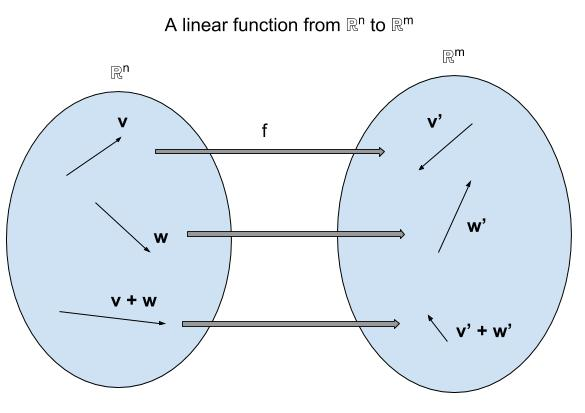
\includegraphics[scale=0.25]{preserving-addition}
\end{center}

\begin{itemize}
\item $f(\bv + \bw) = f(\bv) + f(\bw)$
\item Let $f(\bv) = \bv^{\prime}$.
\item Let $f(\bw) = \bw^{\prime}$.
\item We can compute a vector sum on the left: $\bv + \bw$.
\item We can compute a vector sum on the right: $\bv^{\prime} + \bw^{\prime}$.
\item $f$ must move the vector sum on the left to the vector sum on the right.
\end{itemize}

\end{frame}

\begin{frame}{$f$ Preserves Scalar Multiplication}

\begin{center}
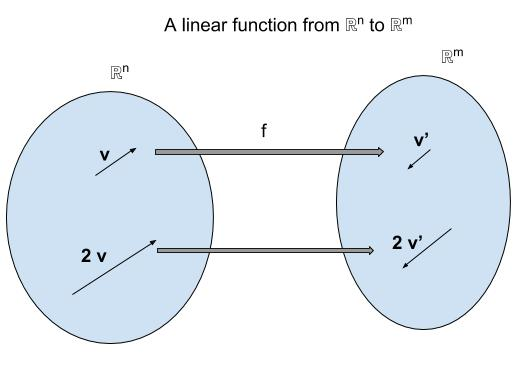
\includegraphics[scale=0.25]{preserving-scalar-mult}
\end{center}

\begin{itemize}
\item $f(c \bv) = c f(\bv)$
\item Let $f(\bv) = \bv^{\prime}$.
\item Let $c = 2$.
\item We can compute a scalar multiplication on the left: $2 \bv$.
\item We can compute a scalar multiplication on the right: $2 \bv^{\prime}$.
\item $f$ must move the scalar multiple on the left to the scalar multiple on the right.
\end{itemize}

\end{frame}

\begin{frame}{Example 1. $f:\R^1\map\R^1$}

\begin{itemize}
\item Let $f:\R^1\map\R^1$ be given by $f(x) = x^2$.
\item Is $f$ linear?
\item Check: Does $f$ preserve vector addition?
\item Note that on $\R^1$ vector addition is just ordinary addition of numbers.
\item $f(x_1 + x_2) = (x_1 + x_2)^2$
\item $= x_1^2 + x_2^2 + 2 x_1 x_2$
\item $= f(x_1) + f(x_2) + 2 x_1 x_2$.
\item So $f(x_1 + x_2) \not= f(x_1) + f(x_2)$
\item unless $2 x_1 x_2 = 0$, i.e. unless $x_1 = 0$ or $x_2 = 0$.
\item So $f$ is \emph{not} linear.
\end{itemize}

\end{frame}

\begin{frame}{Example 1. $f:\R^1\map\R^1$}

\begin{itemize}
\item Continue to let $f:\R^1\map\R^1$ be given by $f(x) = x^2$.
\item We already know $f$ is not linear.
\item Just for fun, check: Does $f$ preserve scalar multiplication?
\item $f(c x) = (c x)^2$
\item $= c^2 x^2$
\item $= c^2 f(x)$.
\item So $f(c x) \not= c f(x)$
\item unless $c^2 = c$, i.e. unless $c=0, 1$.
\item So again, $f$ is not linear.
\end{itemize}

\end{frame}

\begin{frame}{Example 2. $f:\R^1\map\R^1$}

\begin{itemize}
\item Let $f:\R^1\map\R^1$ be given by $f(x) = 2 x$.
\item Is $f$ linear?
\item Check: Does $f$ preserve vector addition?
\item $f(x_1 + x_2) =  2(x_1 + x_2)$
\item $ = 2 x_1 + 2 x_2$
\item $= f(x_1) + f(x_2)$.
\item So $f$ \emph{does} preserve addition.
\item Check: Does $f$ preserve scalar multiplication?
\item $f(c x) = 2 (c x)$
\item $ = c (2 x) $
\item $= c f(x)$.
\item So $f$ does preserve scalar multiplication.
\item So $f$ is linear.
\end{itemize}

\end{frame}

\beamerdefaultoverlayspecification{}

\begin{frame}{Example 3. $f:\R^2\map\R^1$}

\begin{columns}

\column[T]{5cm}
\begin{itemize}
\item<1-> Consider this function from lesson 3:
\item<2-> $f(x,y) = x^2 + y$
\item<3-> Is $f$ linear?
\item<4-> Check: Does $f$ preserve vector addition?
\item<5-> Let $\bv, \bw \in \R^2$
\item<6-> We need to check if $f(\bv + \bw) = f(\bv) + f(\bw)$
\end{itemize}

\column[T]{5cm}
\includegraphics<2->[scale=0.15]{x-squared-plus-y}
\end{columns}

\end{frame}


\begin{frame}{Does $f$ preserve vector addtion?}
\begin{align*}
&f(\bv + \bw) \\
\uncover<2->{&=  f\bigl((v_1, v_2) + (w_1, w_2)\bigr) \\}
\uncover<3->{&= f\bigl(v_1 + w_1, v_2 + w_2\bigr) \\}
\uncover<4->{&= \bigl(v_1 + w_1 \bigr)^2 + (v_2 + w_2) \\}
\uncover<5->{&= (v_1^2 + 2 v_1 w_1 + w_1^2) + (v_2 + w_2) \\}
\uncover<6->{&= (v_1^2 + v_2) + (w_1^2 + w_2)  + 2v_1 w_1\\}
\uncover<7->{&= f(v_1, v_2) + f(w_1, w_2)  + 2v_1 w_1\\}
\uncover<8->{&= f(\bv) + f(\bw)  + 2v_1 w_1\\}
\uncover<9->{&\not= f(\bv) + f(\bw) \text{ unless $v_1=0$ or $w_1=0$}\\}
\end{align*}

\uncover<10->{So $f$ does not preserve vector addtion. So $f$ is not linear.}
\end{frame}

\beamerdefaultoverlayspecification{<+->}

\begin{frame}{Linear Functionals}

\begin{itemize}
\item A linear function from $\R^n$ to $\R^1$ is also called a linear
\emph{functional}.
\item Let $\bv \in \R^n$ be any vector.
\item We will show how $\bv$ can used as a linear functional.
\item In its role as a linear functional, $\bv$ is called a \emph{covector}.
\item Let $f_{\bv} : \R^n \map \R^1$ be defined by
$$f_{\bv}(\bw) = \bv \cdot \bw$$
\item $f_{\bv}$ is called the \emph{covector} associated to the vector $\bv$.
\end{itemize}

\end{frame}

\begin{frame}{Example Covector}

\begin{itemize}
\item Let $\bv = (2, -1)$
\item So $f_{\bv}:\R^2 \map \R$.
\item Let $\bw = (4, 5) \in \R^2$.
\item Compute $f_{\bv}(\bw)$
\item $= \bv \cdot \bw = 8 - 5 = 3$
\item $f_{\bv}(\bw) =  3$.
\end{itemize}

\end{frame}

\begin{frame}{Dot Product is Linear}

\begin{itemize}
\item Claim: For any vector $\bv\in\R^n$, $f_{\bv}:\R^n\map\R$ is linear.
\item proof:
\item First we show that $f_{\bv}$ preserves vector addition.
\item Let $\bu, \bw \in \R^n$
\item We must show $f_{\bv}(\bu + \bw) = f_{\bv}(\bu) + f_{\bv}(\bw)$
\item i.e. that $\bv \cdot (\bu + \bw) = \bv \cdot \bu + \bv \cdot \bw$.
\item This is just the distributive law for dot product.
\end{itemize}

\end{frame}

\beamerdefaultoverlayspecification{}

\begin{frame}{Distributive law for dot product}
\begin{align*}
f_{\bv}(\bu + \bw)
\uncover<2->{&= \bv \cdot (\bu + \bw) }\\
\uncover<3->{&=  \sum_i{v_i (u_i + w_i)} \\}
\uncover<4->{&= \sum_i{v_i u_i +v_i  w_i} \\}
\uncover<5->{&= \sum_i{v_i u_i} + \sum_i{v_i  w_i} \\}
\uncover<6->{&= \bv \cdot \bu + \bv \cdot \bw \\}
\uncover<7->{&= f_{\bv}(\bu) + f_{\bv}(\cdot \bw)}
\end{align*}

\end{frame}

\beamerdefaultoverlayspecification{<+->}

\begin{frame}{Dot Product is Linear (2)}

\begin{itemize}
\item So $f_{\bv}$ preserves vector addition.
\item Now we must show that $f_{\bv}$ preserves scalar multiplication.
\item Let $\bu \in \R^n$ and let $c\in\R$.
\item We must show $f_{\bv}(c \bu) = c f_{\bv}(\bu)$
\item i.e. that $\bv \cdot (c \bu) = c (\bv \cdot \bu)$
\end{itemize}

\end{frame}

\beamerdefaultoverlayspecification{}

\begin{frame}{Dot Product is Linear (3)}
\begin{align*}
f_{\bv}(c \bu)
\uncover<2->{&= \bv \cdot (c \bu) }\\
\uncover<3->{&=  \sum_i{v_i (c u_i)} \\}
\uncover<4->{&= c \sum_i{v_i u_i } \\}
\uncover<5->{&= c (\bv \cdot \bu) \\}
\uncover<5->{&= c f_{\bv}(\bu)}
\end{align*}

\end{frame}

\beamerdefaultoverlayspecification{<+->}

\begin{frame}{Dot Product is Linear (4)}

\begin{itemize}
\item So $f_{\bv}$ preserves scalar multiplication.
\item So $f_{\bv}$ is linear. $\qed$.
\end{itemize}

\end{frame}

\begin{frame}{Linear functions preserve linear combinations}
\begin{lemma}
Let $f:\R^n\map\R^m$. The following are equivalent:
\begin{enumerate}
\item $f$ is linear
\item $f$ preserves all linear combinations.

\pause

i.e. for every
$\bw_1,\bw_2,\cdots\bw_k\in\R^n$, for every $c_1,c_2,\cdots c_k\in\R$,
$$f(c_1 \bw_1 + c_2 \bw_2 + \cdots + c_k \bw_k) = c_1 f(\bw_1) + c_2 f(\bw_2) + \cdots + c_k f(\bw_k)$$

\pause

\item $f$ preserves linear combinations of length 2.

\pause

i.e. for every $\bw_1,\bw_2\in\R^n$, for every $c_1,c_2\in\R$,
$f(c_1 \bw_1 + c_2 \bw_2) = c_1 f(\bw_1) + c_2 f(\bw_2) f(\bw_k)$.

\end{enumerate}
\end{lemma}
\end{frame}


\begin{frame}{Example: Covector preserves linear combinations}

\begin{itemize}
\item Let $\bv = (2, -1)$
\item So $f_{\bv}:\R^2 \map \R$.
\item Let $\bw_1 = (4, 5) \in \R^2$.
\item Let $\bw_2 = (1,-1) \in \R^2$.
\item $f_\bv(2\bw_1 -3\bw_2)$
\item $=f_\bv\bigl((5, 13)\bigr)$
\item $=\bv \cdot (5, 13)$
\item $=10 - 13 = -3$.
\item $2 f_{\bv}(\bw_1) -3 f_{\bv}(\bw_2)$
\item $= 2 (\bv \cdot \bw_1) -3 (\bv \cdot \bw_2)$
\item $=2 (3) - 3(3)$
\item $=-3$
\item So $f_\bv(2\bw_1 -3\bw_2) = 2f_{\bv}(\bw_1) -3 f_{\bv}(\bw_2)$.
\end{itemize}

\end{frame}

\begin{frame}{Proof of Lemma}

\begin{itemize}
\item (3) $\implies$ (1). Suppose that $f$ preserves linear combinations of length 2.
\item $f(c_1 \bw_1 + c_2 \bw_2) = c_1 f(\bw_1) + c_2 f(\bw_2)$.
\item Letting $c2=0$ we have
\item $f(c_1 \bw_1) = c_1 f(\bw_1)$.
\item So $f$ preserves scalar multiplication.
\item Letting $c_1 = c_2 = 1$ we have
\item $f(\bw_1 + \bw_2) = f(\bw_1) + f(\bw_2)$.
\item So $f$ preserves vector addition.
\item So $f$ is linear.
\item (2) $\implies$ (3) is trivial. So we are left with...
\item (1) $\implies$ (2). Suppose $f$ is linear.
\item We must show that $f$ preserves all linear combinations.
\item This is done by induction on $k$.
\item The base case, $k=1$, says $f(c_1 \bw_1) = c_1 f(\bw_1)$.
\item This follows from the fact that $f$ preserves scalar mult.
\end{itemize}

\end{frame}

\beamerdefaultoverlayspecification{}

\begin{frame}{The inductive step}
Now suppose that
$$f\left(\Sigma_{i=1}^k{c_i \bw_i}\right) = \Sigma_{i=1}^k{c_i f(\bw_i)}$$

\smallskip

We must show that
$$f\left(\Sigma_{i=1}^{k+1}{c_i \bw_i}\right) = \Sigma_{i=1}^{k+1}{c_i f(\bw_i)}$$

\begin{align*}
&f\left(\Sigma_{i=1}^{k+1}{c_i \bw_i}\right)\\
\uncover<2->{&=  f\left(\Sigma_{i=1}^{k}{c_i \bw_i} + c_{k+1} \bw_{k+1}\right)\\}
\uncover<3->{&=  f\left(\Sigma_{i=1}^{k}{c_i \bw_i}\right) + f(c_{k+1} \bw_{k+1}) \quad \text{ ($f$ preserves addition)} \\}
\uncover<4->{&= \Sigma_{i=1}^k{c_i f(\bw_i)} + f(c_{k+1} \bw_{k+1}) \quad \text{ (induction)}\\}
\uncover<5->{&= \Sigma_{i=1}^k{c_i f(\bw_i)} + c_{k+1} f(\bw_{k+1}) \quad \text{ ($f$ preserves scalar mult.)}\\}
\uncover<6->{&= \Sigma_{i=1}^{k+1}{c_i f(\bw_i)} }
\end{align*}

\uncover<7->{So $f$ preserves all linear combinations. $\qed$.}
\end{frame}

\beamerdefaultoverlayspecification{<+->}

\begin{frame}{Arbitrary functions are flexible}
\begin{itemize}
\item Suppose $f:\R^2\map\R$ is \emph{some} function. (Not necessarily linear).
\item Suppose I told you that $f(0,1) = 12$
\item and I told you that $f(1, 0) = -1$.
\item Question: What is $f(2, 2)$?
\item Answer: You have no idea. It could be anything.
\item Arbitrary functions are "flexible". They can bend however you want them to.
\item Knowing the value of $f$ at any finite number of points tells you nothing
about the value of $f$ at any other point.
\item Now suppose I told you $f$ were linear?
\item Then $f(2,2) = f\left(2(1,0) + 2(0,1)\right)$
\item $=2f(1,0) + 2f(0,1)$
\item $= 2(12) + 2 (-1) = 23$.
\end{itemize}
\end{frame}

\beamerdefaultoverlayspecification{}

\begin{frame}{Values at the standard basis vectors}

A linear function is determined by its values at the standard basis vectors.

\uncover<2->{
\begin{lemma}
Let $f:\R^n\map\R^m$ and $g:\R^n\map\R^m$  be two linear functions. \\
\uncover<3->{Suppose that $f(\be_i) = g(\be_i)$ for $i=1, 2, \cdots n$.} \\
\uncover<4->{Then $f = g$.}
\end{lemma}
}

\end{frame}

\begin{frame}{Proof of Lemma}

\begin{proof}
Assume $f(\be_i) = g(\be_i)$ for $i=1, 2, \cdots n$.
Let $\bv\in\R^n$ be any vector.
\uncover<2->{We must show that $f(\bv)=g(\bv)$.}
\uncover<3->{
Now $\bv = (v_1,v_2,\cdots v_n)$.
So $\bv=\sum_i{v_i \be_i}$.
}

\begin{align*}
\uncover<4->{f(\bv) &= f\left(\sum_i{v_i \be_i}\right) \\}
\uncover<5->{&= \sum_i{v_i f(\be_i)} \text{ \qquad (by linearity)}\\}
\uncover<6->{&= \sum_i{v_i g(\be_i)} \text { \qquad (by assumption)}\\}
\uncover<7->{&= g\left(\sum_i{v_i \be_i}\right) { \qquad  (by linearity)} \\}
\uncover<8->{&= g(\bv)}
\end{align*}
\end{proof}
\end{frame}

\beamerdefaultoverlayspecification{<+->}

\begin{frame}{All functionals are covectors}

All functionals on $\R^n$ are given by covectors.

\pause

\begin{lemma}
Let $f:\R^n\map\R$ be a covector.\\
\pause
Then there is a vector $\bv\in\R^n$ such that $f=f_{\bv}$. \\
\end{lemma}

\pause

\begin{itemize}
\item Proof:
\item Let $a_i = f(\be_i)$ for $i=1,\cdots n$.
\item Let $\bv=(a_1, a_2, \cdots a_n)$.
\item Notice $\bv\cdot\be_i=a_i$ for $i=1,\cdots n$.
\item So $f_{\bv}(\be_i)=a_i$ for $i=1,\cdots n$.
\item So $f_{\bv}(\be_i)=f(\be_i)$ for $i=1,\cdots n$.
\item By the previous lemma, $f = f_{\bv}$. $\qed$
\end{itemize}

\end{frame}

\begin{frame}{Linear component functions}

A function is linear iff it's component functions are.

\pause

\begin{lemma}
Let $f:\R^n\map\R^m$ be a function.\\
\pause
Write $f(\bv) = \left(f_1(\bv),f_2(\bv),\cdots f_m(\bv)\right)$. \\
\pause
Then the following are equivalent:
\pause
\begin{enumerate}
\item $f$ is linear
\item $f_i$ is linear for $i=1,\dots m$.
\end{enumerate}
\end{lemma}

\pause

\begin{itemize}
\item Proof:
\item Let $\bv_1,\dots\bv_n\in\R^n$ and let $c_1,\dots c_n \in\R$.
\item $f\left(\sum_j{c_j \bv_j}\right) = \sum_j{c_j f(\bv_j)}$
\item iff $\left(f_1\left(\sum_j{c_j \bv_j}\right),\cdots,f_m\left(\sum_j{c_j \bv_j}\right)\right) = \left( \sum_j{c_j f_1(\bv_j)},\cdots \sum_j{c_j f_m(\bv_j)} \right)$
\item iff $f_i\left(\sum_j{c_j \bv_j}\right) = \sum_j{c_j f_i(\bv_j)}$, for $i=1,\dots m$.
\end{itemize}

\end{frame}

\begin{frame}{Characterization of linear functions}

All linear functions from $\R^n$ to $\R^m$ are given by $m$ covectors.

\pause

\begin{theorem}
Let $f:\R^n\map\R^m$ be a linear function.\\
\pause
Then there are $m$ vectors $\bv_1,\bv_2,\cdots\bv_m \in \R^n$ such that
$f = \left(f_{\bv_1}, f_{\bv_2}, \cdots f_{\bv_m}\right)$.

\pause
\smallskip

Conversely, Let $\bv_1,\bv_2,\cdots\bv_m$ be any $m$ vectors in $\R^n$ and
let $f=\left(f_{\bv_1}, f_{\bv_2},\cdots f_{\bv_n}\right)$.
\pause
Then $f:\R^n\map\R^m$ is linear.

\end{theorem}

\end{frame}

\begin{frame}{Proof of theorem}

\begin{itemize}
\item Let $f:\R^n\map\R^m$ be a linear function.
\item Write $f = (f_1, f_2, \cdots f_m)$.
\item From a previous lemma each $f_i$ is linear.
\item But $f_i:\R^n\map\R$ so each $f_i$ is a linear functional.
\item But all linear functionals are covectors.
\item So for each $i$, let $\bv_i$ be such that $f_i = f_{\bv_i}$.
\item Then $f=(f_{\bv_1}, f_{\bv_2},\cdots f_{\bv_n})$.
\item Conversely, let $\bv_1,\bv_2,\cdots\bv_m$ be any $m$ vectors in $\R^n$.
\item Let $f=(f_{\bv_1}, f_{\bv_2},\cdots f_{\bv_n})$.
\item Since each of the component functions of $f$ is linear, $f$ is linear.
\end{itemize}


\end{frame}

\begin{frame}{Example: A linear $f:\R^2\map\R^3$}
According to the theorem, a linear function from $\R^2$ to $\R^3$ is
given by three covectors from $\R^2$.

\begin{itemize}
\item Let $\bv_1 = (2, 1)$
\item Let $\bv_2 = (0, -3)$
\item Let $\bv_3 = (-1, 0)$
\item Let $f = (f_{\bv_1},f_{\bv_2},f_{\bv_3})$.
\item Then $f:\R^2\map\R^3$ is linear.
\item Let $\bw = (3, -2)$. Compute $f(\bw)$.
\item $f(\bw) = \left(f_{\bv_1}(\bw),f_{\bv_2}(\bw),f_{\bv_3}(\bw)\right)$
\item $=(4, 6, -3)$
\end{itemize}

\end{frame}

\begin{frame}{Composition of linear functions}

The composition of linear functions is linear.

\pause

\begin{lemma}
Let $f:\R^n\map\R^m$ be linear. Let $g:\R^m\map\R^k$ be linear.
Let $h:\R^n\map\R^k$ be given by $h=g\circ f$.
\pause
Then $h$ is linear.
\end{lemma}

\pause

proof:

\begin{itemize}
\item $h(a\bv +b\bw)$
\item $= g(f(a\bv +b\bw))$
\item $= g(a f(\bv) + b f(\bw))$ \quad (because $f$ is linear)
\item $= a g(f(\bv)) + b g(f(\bw))$ \quad (because $g$ is linear)
\item $= a h(\bv) + b h(\bw)$.
\item So $h$ is linear. $\qed$.
\end{itemize}

\end{frame}

\begin{frame}{Example Composition}

Let $f:\R^2\map\R^3$ be the function we considered a few slides back:

\begin{itemize}
\item Let $\bv_1 = (2, 1)$
\item Let $\bv_2 = (0, -3)$
\item Let $\bv_3 = (-1, 0)$
\item Let $f = (f_{\bv_1},f_{\bv_2},f_{\bv_3})$.
\item So $f:\R^2\map\R^3$ is linear.
\item Now let $\bu\in\R^3 = (-1, -1, 2)$.
\item Then $g = f_{\bu}:\R^3\map\R$ is a covector from $\R^3$.
\item Now let $h=g\circ f$.
\item Then $h:\R^2\map\R^1$. According to the theorem it is linear.
\item Let $\bw = (3, -2)$. Compute $h(\bw)$.
\item From our earlier example $f(\bw) =(4, 6, -3)$.
\item So $h(\bw) = g(4, 6, 3)$ = $\bu\cdot(4,6,3) = -4 -6 -6 = -16$.
\end{itemize}

\end{frame}

\begin{frame}{Operations on linear functions}

We can consider the \emph{set of all} linear functions from $\R^n$ to $\R^m$.

\begin{itemize}
\item Let $L(\R^n,\R^m)$ mean the set of all linear functions from $\R^n$ to $\R^m$.
\item There are a few \emph{operations} that make sense on $L(\R^n, \R^m)$.
\item Addition:
\item Let $f, g \in L(\R^n, \R^m)$. We can define $f+g$.
\item Scalar multiplication:
\item Let $f\in L(\R^n, \R^m)$. Let $c\in\R$. We can define $cf$.
\end{itemize}

\end{frame}

\begin{frame}{Addition of linear functions}

\begin{itemize}
\item Let $f, g \in L(\R^n,\R^m)$.
\item We want to define $h = f+g \in L(\R^n,\R^m)$.
\item Now $f:\R^n\map\R^m$ and $g:\R^n\map\R^m$.
\item We want to define $h:\R^n\map\R^m$.
\item How should we define $h$?
\item Let $\bv\in\R^n$. What should $h(\bv)$ be?
\item $h(\bv) = (f+g)(\bv) = ?$
\item $=f(\bv) + g(\bv)$.
\end{itemize}

\end{frame}

\begin{frame}{Sum of linear functions is linear}

\begin{lemma}
Let $f,g\in L(\R^n, \R^m)$. Then $f+g$ is linear.
\end{lemma}

\pause

Proof:

\pause

\begin{itemize}
\item $(f+g)(c_1 \bv_1 + c_2 \bv_2)$
\item $=f(c_1 \bv_1 + c_2 \bv_2) + g(c_1 \bv_1 + c_2 \bv_2)$ \quad (Definition of $f+g$)
\item $=c_1f(\bv_1)+ c_2f(\bv_2) + c_1g(bv_1) + c_2g(\bv_2)$ \quad ($f$ and $g$ are both linear)
\item $= c_1\left(f(\bv_1)+  g(bv_1)\right) + c_2\left(f(\bv_2) + g(\bv_2)\right)$
\item $=c_1\left((f + g)(\bv_1)\right) + c_2\left((f+g)(\bv_2) \right)$ \quad (Definition of $f+g$)
\end{itemize}

\pause

So $f+g$ is linear. $\qed$.

\end{frame}

\begin{frame}{Scalar multiplication of linear functions}

\begin{itemize}
\item Let $f \in L(\R^n,\R^m)$. Let $c\in\R$.
\item We want to define $h = c f \in L(\R^n,\R^m)$.
\item Now $f:\R^n\map\R^m$.
\item We want to define $h:\R^n\map\R^m$.
\item How should we define $h$?
\item Let $\bv\in\R^n$. What should $h(\bv)$ be?
\item $h(\bv) = (c f)(\bv) = ?$
\item $= c \left(f (\bv)\right)$.
\end{itemize}

\end{frame}

\begin{frame}{Scalr multiple of a linear function is linear}

\begin{lemma}
Let $f\in L(\R^n, \R^m)$. Let $c\in\R$. Then $c f$ is linear.
\end{lemma}

\pause

Proof:

\pause

\begin{itemize}
\item $(c f)(c_1 \bv_1 + c_2 \bv_2)$
\item $=c \left (f(c_1 \bv_1 + c_2 \bv_2) \right )$ \quad (Definition of $c f$)
\item $= c \left(c_1 f(\bv_1) + c_2 f(\bv_2)  \right)$ \quad ($f$ is linear)
\item $= \left(c_1 \cdot c \cdot f(\bv_1) + c_2 \cdot c \cdot f(\bv_2)  \right)$
\item $= \left(c_1 (c f)(\bv_1) + c_2 (c f)(\bv_2)  \right)$ \quad (Definition of $c f$)
\end{itemize}

\pause

So $c f$ is linear. $\qed$.

\end{frame}

\end{document}


